在我们理解了仿射概形后,射影概形\index{射影!概形}的理论并不会包含太多新奇的东西:在大多数情况下,它与射影簇的经典理论的差别完全类似于仿射概形和仿射簇的经典理论之间的差别。

我们首先将引入两个有限性条件,\textit{有限}以及\textit{有限型},然后定义和讨论\textit{分离}以及\textit{逆紧}态射\index{逆紧!态射},它们分别对应于绝大多数几何中的Hausdorff性与紧性。而正是部分因为射影簇和概形有这些性质,它们才是经典代数几何以及概形理论的基本研究对象。

这章的下一部分将引入射影概形以及给出一些例子。如同仿射概形的情形,有两种入手射影概形的法子:一种是定义出射影空间然后取它们的子概形,另一种是将所有的射影概形建立在同一个根基上,从分次代数入手。正如处理仿射情况那般,这里我们采用第二种方法。

在介绍了射影概形的基础定义以及它们的子概形后,我们将描述射影概形之间的态射,相较于仿射对应,它将更加微妙而难以捉摸(就像在簇范畴中那样)。我们将用一些射影概形的例子结束这节,其中最值得注意的是Grassmann流形。

本章的最后一节将给出嵌入在射影空间中的射影概形的三个不变量,它们由David Hilbert所引入:Hilbert多项式、Hilbert函数以及自由分解(free resolution). 使用它们,我们有时能区分类似的概形,比如射影双重直线,以及可以
揭示平坦性的一些新现象。在一个射影概形的不变量中,可以根据其Hilbert多项式定义的不变量的是它的度数;在这方面的联系,我们将讨论著名的B\'{e}zout定理。

\section{一些态射的性质}\label{s:3.1}

\subsection{有限性条件}\label{s:3.1.1}

在大多数有关概形的非平凡结论中,有两个有限性条件。它们有着相似的名字但非常不同的性质。第一个有限性条件,有限型,是一个在绝大多数几何背景中产生的态射都满足的直截了当的性质,他被引入常是为了排除无穷维的纤维或者“非几何”的概形,比如局部环的谱。而另一个有限性条件,有限,比较起来就是一个非常严格的条件:它是说一个态射是逆紧的以及它的所有纤维都是有限的(特别地,零维的)。

首先,我们称一个概形间的态射$\varphi:X\to Y$是\textit{有限型}的,如果对每一点$y\in Y$,都存在一个$y$的仿射开邻域$V=\spec B\subset Y$使得它的原像被一族仿射开集$U_i\cong \spec A_i$有限覆盖,即
\[
	\varphi^{-1}(V)=\bigcup_{i=1}^n U_i,
\]
并且在映射
\[
	\varphi_V^\#:B=\oo_Y(V)\to \oo_X (\varphi^{-1}V)\to \oo_X(U_i)=A_i
\]
下,每个$A_i$都是一个有限生成$B$\hyp 代数。因此,比如,任意$\mathbb{A}_K^n$或$\mathbb{P}_K^n$的子概形是在$K$上有限型的(意思是,结构态射$X\to \spec K$是有限型的),而一个正维数的局部$K$\hyp 代数的谱不是。

一个态射$\varphi:X\to Y$被称为\textit{有限}\index{有限}的,如果对每点$y\in Y$都有它的一个开仿射邻域$V=\spec B\subset Y$使得原像$\varphi^{-1}(V)=\spec A$也是仿射的,以及通过拉回
\[
	\varphi_V^\#: B =\oo_Y(V)\to \oo_X(\varphi^{-1}V)=A,
\]
$A$是一个有限生成$B$-模。这是一个比有限型更强的条件,首先,马上可以由其给出$\varphi$的纤维是有限的,其次,拓扑空间之间的映射$|\varphi|:|X|\to |Y|$是一个闭映射。因此,对$Y=\spec B$以及多项式$f\in B[x]$,如果$f$的最高项系数是一个可逆元但其他不是,则态射$\spec(B[x]/(f))\to Y$是有限的。这些都可以参考 Eisenbud [1995, Chapter 4 and Section 9.1].

\subsection{逆紧性和分离性}\label{s:3.1.2}

许多几何上的技术应用于紧Hausdorff空间时可以获得最完整的结果。尽管仿射概形在Zariski拓扑下是预紧的,但是它们并不共享在其他理论中紧空间的良好属性,因为Zariski拓扑不是Hausdorff的。举个例子,即使$X$是预紧的,仿射概形间的正则映射$\varphi:X\to Y$的像也可能不是闭的。

Zariski拓扑并不Hausdorff这点还有着其他令人不爽的结果。回忆在流形的一般定义中,我们从一个Hausdorff空间开始,在它上面装备一个坐标卡的覆盖,坐标卡是一个标准型(即欧式空间中的球)。但注意到,即使这些球都是Hausdorff的,也不足以说明整个空间是Hausdorff的。这就是为什么在Exercise \ref{exe:1.44} 中描述的具有双重原点的直线(这里重新展示如下)

\begin{center}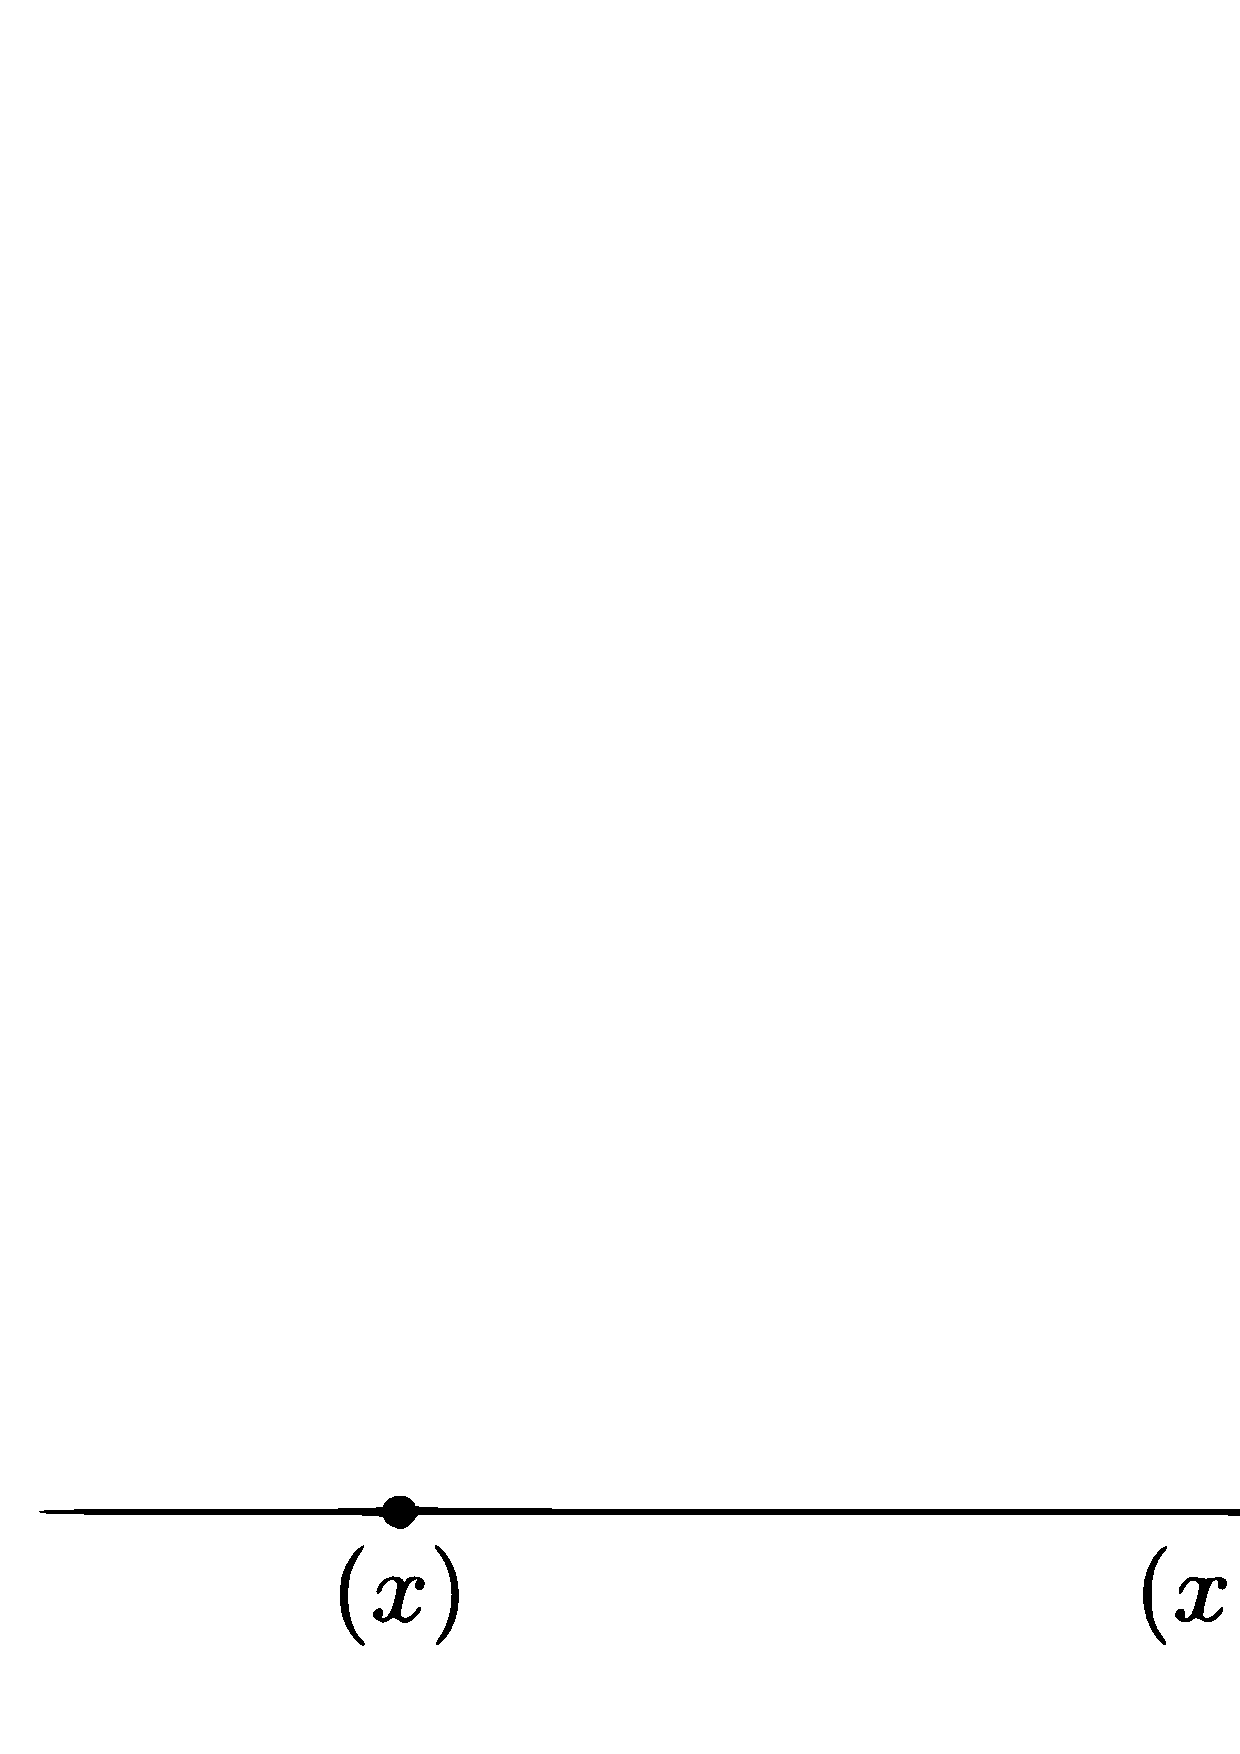
\includegraphics[scale=\scale,bb=0 0 562 68]{\PICDIR/1.png}\end{center}

\vspace{-0.4em}\noindent 不是一个流形。然而,当我们处理由仿射概形拼成的概形(或者簇)的时候,我们不能指定整个空间是Hausdorff的,因为即使就局部来说,那些拼合的部件也不是Hausdorff的。于是,对给定两个概形之间的两个态射$\varphi$, $\psi:X\to Y$,$\varphi$和$\psi$相等的点构成的集并不会是闭的。下面习题中的典型例子将展示这点。

\begin{exe}
\begin{compactenum}[(a)]
\item 令$Y$是在域$K$上的具有双重原点的直线,正如在Exercise \ref{exe:1.44} 中的定义,以及令$\varphi_1$, $\varphi_2:\mathbb{A}_K^1\to Y$是两个显然的含入映射,证明$\varphi_1$和$\varphi_2$相等的点(仅作为拓扑空间间的连续映射)构成的集合不是闭的。
\item 现在令$X=Y\times_K Y$以及$\varphi$和$\psi$分别是两个到$X$到$Y$的典范投射。证明,$\varphi$和$\psi$相等的点构成的集合不是闭的(注意到这就是下面要定义的对角线)。证明,使得$\varphi$和$\psi$相等的闭点构成的集合也不是闭的。所以,这个病态现象并不是概形特有的,它在簇范畴中已经出现了。
\end{compactenum}
\end{exe}

然而,这样的病态现象在$X$是一个仿射概形时并不会出现,同样,当$X$是一个射影概形的时候,这样的事情也被证实是不会出现的。这些概形所具有的理想性质,正是对应的流形上Hausdorff性的最重要结果之一(分离性),它表为:$X$作为一个概形在$K$上是\textit{分离的}。一般地,给定概形间的任意的映射$\alpha:X\to S$,我们定义\textit{对角}子概形$\Delta\subset X\times_S X$如下:局部地,在$X\times_S X$的每一个仿射开集上
\[
	X\supset \spec A\xrightarrow{\alpha|_{\spec A}}\spec B\subset S,
\]
它由所有形如
\[
a\otimes 1 - 1\otimes a \in A\otimes_B A
\]
的元素生成的理想$I$所定义。接着,我们称$\alpha$是\textit{分离的},或者说$X$是\textit{在$S$上分离的概形},如果$\Delta$是$X\times_S X$的一个闭子概形。

\begin{exe}
令$Y\to S$是拓扑空间之间的一个映射,然后令
\[
	\Delta \subset Y\times_S Y
\]
是其对角。证明,如果$\Delta$是一个闭集,那么对任意的交换图
\[
	\xymatrix{
		X\ar@<0.3ex>[rr]^\varphi \ar@<-0.3ex>[rr]_\psi\ar[dr] &&Y\ar[ld]\\
		&S&
	}
\]
$X$中使得$\varphi$和$\psi$相等的点集是一个闭集。现在证明对概形正则映射的相似引理:证明,存在一个自然定义的(即,极大的)闭子概形使得限制在上面$\varphi$和$\psi$是相同的。
\end{exe}

\begin{exe}
	令$X$是一个在$S$上分离的概形。证明$X$的(闭或开)子概形依然在$S$上分离。
\end{exe}

\begin{exe}
	注意,从对角子概形的定义来看,仿射态射是分离的。
\end{exe}

我们在下面将看到射影概形(等等就会定义)同样是分离的,因此,至少这些Hausdorff空间的性质对它们也是成立的。

在经典的仿射簇的情形中(即使简单如平面曲线),在上个世纪初就意识到,得到一些表现得像一个紧的对象的东西(实际上,在复数域上的仿射簇的情形中,在通常的拓扑下就是紧的),最简单的方式是取一个仿射簇在射影空间中的闭包。事实证明,如果$\varphi:X\to Y$是一个射影簇之间的映射,那么$\varphi$确实会将$X$的闭子簇映成$Y$的闭子簇。稍一般些,如果我们取这样一个映射以及一个任意的簇$Z$,得到
\[
	\psi:=\varphi\times 1_Z:X\times Z\to Y\times Z,
\]
则$\psi$将$X\times Z$的闭子簇映到$Y\times Z$的闭子簇。事实证明,\textit{这个性质连同分离性是使得射影概形如此有用的核心性质}。但是,满足这性质的簇要比射影簇稍多,且这个性质有时比起射影性更容易验证,所以给一个更一般的定义很重要。

如果$\alpha:X\to S$是一个概形之间的有限型映射,如果$\alpha$是可分的且对所有的映射$T\to S$,纤维积的投影
\[
	X\times_S T\to T
\]
将闭子集变成闭子集,则称$\alpha$是\textit{逆紧的},或者说$X$\textit{在$S$上逆紧}。同前,如果$S=\spec R$是一个环,我们时常会说“在$R$上逆紧”来意指“在$\spec R$上逆紧”。

上面对$\alpha$在分离性外给出的条件时常被叫做$\alpha$是\textit{全景闭的}。\textit{逆紧}这个名字来自一个旧的几何概念:一个Hausdorff空间之间的映射$\alpha:M\to N$被称为逆紧的如果每一个紧集的原像都是紧的。这是映射$\alpha$的一种相对紧性。这个性质与我们的定义之间的联系见下面的习题。

\begin{exe}
令$\mathscr C$是具有可数拓扑基的局部紧Hausdorff空间构成的范畴。证明映射$f:X\to Y$在$\mathscr C$中是全景闭的当且仅当他是逆紧的,即对任意的$Y$中的紧集$C$,$f^{-1}(C)$也是紧的。
\end{exe}

不管对于概形还是对于簇,逆紧这个概念已被证明是代数几何中的关键性质,它起到了其他几何理论中“紧且Hausdorff”的作用。下面我们将引入的射影概形是最一般的在给定概形$B$上逆紧的概形的例子。我们这里不会证明这个关键的结论,它并不是很难,但是将把我们引开太远。证明可以参见,比如,Hartshrone [1977, Theorem II.4.9].

一个有限态射$\varphi:X\to Y$当然是逆紧的,见Eisenbud [1995, Section 4.4].
